\documentclass[twocolumn]{article}
\usepackage[margin=0.5in]{geometry}
\usepackage{graphicx}
\usepackage{nonfloat}
\usepackage{empheq}
\usepackage{amsmath}
\usepackage{amssymb}
\usepackage{amsfonts}
\usepackage{bbold}
\usepackage{cancel}
\usepackage[plain]{algorithm}
\usepackage[noend]{algpseudocode}

%%%%%%%%

\newcommand\myfigure[1]{%
\medskip\noindent\begin{minipage}{\columnwidth}
\centering%
#1%
%figure,caption, and label go here
\end{minipage}\medskip}

%%%%%%%%

\begin{document}

\section{Asymptotic analysis}
\begin{itemize}
\item Notations
  \begin{itemize}
  \item $O(f(x))$: upper bound.
  \item $\Omega(f(x))$: lower bound.
  \item $\Theta(f(x))$: both upper and lower bound.
  \item Not every $g(x)$ has $\Theta(f(x))$.
    \begin{itemize}
    \item $g(x) = (1 + \sin x) x^3 + x^2$
    \end{itemize}
  \end{itemize}
\item Master theorem
  \begin{itemize}
  \item $T(n) = a T(n/b) + f(n)$, $a \ge 1, b > 1$
  \item Case 1: $f(n) = O(n^c)$, $c < \log_b a$.\\
  Then $T(n) = \Theta(n^{\log_b a})$.
    \begin{itemize}
    \item Example: $T(n) = 8 T(n/2) + 10 n^2$.\\
    $a = 8, b = 2, c=2, \log_b a = 3 > c$.\\
    Thus $T(n) = \Theta(n^3)$
    \end{itemize}
  \item Case 2: $f(n) = \Theta(n^c \log^k n)$, $c=\log_b a$.\\
  Then $T(n) = \Theta(n^c log^{k+1} n)$.
    \begin{itemize}
    \item Example: $T(n) = 2 T(n/2) + 10 n$.\\
    $a=2, b=2, c=1, k=0, \log_b a = 1 = c$.\\
    Thus $T(n) = \Theta(n \log n)$
    \end{itemize}
  \item Case 3: $f(n) = \Omega(n^c)$, $c > \log_b a$.\\
  Then $T(n) = \Theta(f(n))$.
    \begin{itemize}
    \item Example: $T(n) = 2 T(n/2) + n^2$.\\
    $a=2, b=2, c=2, \log_b a = 1 < c$.\\
    Thus $T(n) = \Theta(n^2)$
    \end{itemize}
  \end{itemize}
\end{itemize}

\section{Divide and conquer}
\begin{itemize}
\item Example: peak finding
  \begin{itemize}
  \item 1-d [$O(\lg n)$]:
    \begin{itemize}
    \item a[m-1] $>$ a[m]: search left.
    \item a[m+1] $>$ a[m]: search right.
    \end{itemize}
  \item 2-d [$O(n \lg n)$]:
    \begin{itemize}
    \item Given $m$th col, find max in $i$th row.
    \item a[i, m-1] $>$ a[i, m]: search left.
    \item a[i, m+1] $>$ a[i, m]: search right.
    \end{itemize}
  \end{itemize}

\end{itemize}
    
\section{Heap}
\begin{itemize}
\item Priority queue
  \begin{itemize}
  \item insert(S, x)
  \item max(S)
  \item extract\_max(S)
  \item increase\_key(S, x, k)
  \end{itemize}
\end{itemize}

\subsection{Max heap}
  \begin{itemize}
  \item Parent is greater than children (and descendants).
  \item build\_max\_heap[$O(n)$]: bottom up max\_heapify.
    \\Denote $h$ as height. $\frac{n}{4}$th node has height $1$.
    \begin{align*}
    T(n) = \sum_{h=1}^{H} \frac{n}{2^{h+1}} \, h = \frac{n}{2} \sum_{h=1}^H \frac{h}{2^h} = O(n)
    \end{align*}
    $\sum_{l=0}^{\infty} h x^h = \frac{x}{(1-x)^2}$ when $x<1$. Here $x = 1/2$.
    \begin{gather*}
    s = \sum_{h=0}^{\infty} h x^h
    \\
    t = \int \frac{s}{x} dx = x \sum_h x^h = \frac{x}{1-x}
    \\
    \frac{s}{x} = \frac{dt}{dx} = \frac{1}{(1-x)^2}
    \end{gather*}
  \item max\_heapify[$O(\log h)$]: sink down a node, provided this node is not max heap, but both children are max heap. This process makes the node a max heap. 
  \item insert[$O(\log H)$]: insert to the end and bubble up.
  \item pop[$O(\log H)$]: replace root with last and heapify.
  \end{itemize}
  
%%%%

\subsection{Median heap}
\begin{itemize}
\item Maintain MaxHeap on the left and MinHeap on the right.
\item Insert:
  \begin{itemize}
  \item Insert into MaxHeap, if key $<$ root of MaxHeap.
  \item Insert into MinHeap, otherwise.
  \item Balance if $size_{max} - size_{min} > 1$ by pop-and-insert.
  \end{itemize}
\end{itemize}

%%%%%%%%

\section{Tree}
\begin{itemize}
\item Height of tree: length of longest path from root to leaf.
\item Height of node: length of longest path from node to leaf.
\item Depth of node: length from root to node.
\item Augmented tree: augment nodes with some property (size, height, etc.).
\item Balanced tree: $h = O(\lg n)$.
  \begin{itemize}
  \item AVL tree
  \item Red-black (2-3-4) tree
  \item Skip list
  \item Treap
  \item 2-3 tree
  \item B-tree
  \end{itemize}
\end{itemize}

%%%%

\subsection{Binary search tree}
\begin{itemize}
\item Example: lane reservation.
\item Def: left is smaller, right is larger.
  \item search, min, max [$O(h)$]
  \item succ [$O(h)$]
    \begin{itemize}
    \item Case 1: has right child.
    \item Case 2: doesn't have right child.
    \end{itemize}
    \begin{figure}[H]
    \centering
    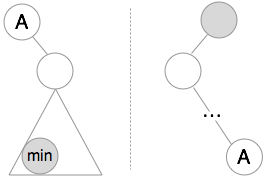
\includegraphics[width=0.3\textwidth]{assets/bst-succ}
    \end{figure}
  \item pred [$O(h)$]
    \begin{figure}[H]
    \centering
    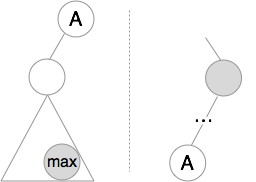
\includegraphics[width=0.3\textwidth]{assets/bst-pred}
    \end{figure}
  \item insert
    \begin{itemize}
    \item Probe parent.
    \item Insert node as leaf.
    \end{itemize}
  \item delete
    \begin{itemize}
    \item Transplant
      \begin{itemize}
      \item Carry
        \begin{figure}[H]
        \centering
        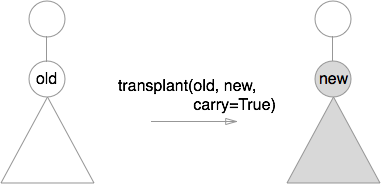
\includegraphics[width=0.42\textwidth]{assets/bst-transplant-carry}
        \end{figure}
      \item Non-carry
        \begin{figure}[H]
        \centering
        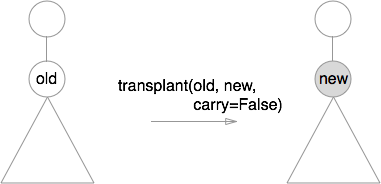
\includegraphics[width=0.42\textwidth]{assets/bst-transplant-ncarry}
        \end{figure}
      \end{itemize}
    \item Case 1: node with single left (or nill).
    \item Case 2: node with single right (or nill).
    \item Case 3: node with both children.
    \item Candidate strategy:
    \begin{itemize}
      \item Case 1/2: transplant its only child.
	  \item Case 3, strategy 1: transplant min of right subtree. Min of right subtree falls into case 1 or 2, and needs one more transplant.
      \item Case 3, strategy 2: transplant max of left subtree. Max of left subtree falls into case 1 or 2, and needs one more transplant.
    \end{itemize}
    \begin{figure}[H]
    \centering
    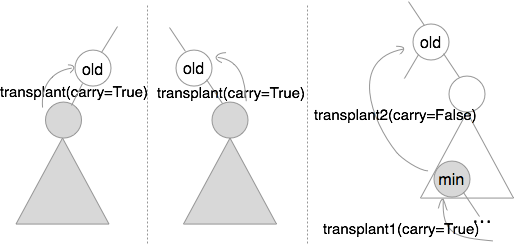
\includegraphics[width=0.48\textwidth]{assets/bst-delete}
    \end{figure}
    \end{itemize}
\end{itemize}

%%%%

\subsection{AVL tree}
\begin{itemize}
\item Def: $|h_{left} - h_{right}| \le 1,\ \  (h_{null} = -1)$.

\item AVL tree is balanced tree. Proof: Denote $N_h$ as min \# of nodes to form an AVL tree, then
  \begin{align*}
  N_h &= 1 + N_{h-1} + N_{h-2}
  \\&> 2 N_{n-2} = \Theta(2^{h/2})
  \\
  h &= \Theta(\lg N_h) = O(\lg n)
  \end{align*}

\item insert
  \begin{itemize}
  \item Intuitions:
    \begin{itemize}
    \item left\_rotate on the right-heavy node.
    \item right\_rotate on the left-heavy node.
    \item Only ancestors of the inserted node can become unbalanced after insertion.
    \item Ensure only ancestors need rotation, and keep subtrees untainted.
    \end{itemize}
  \item left\_rotate: rotate node from parent to left child.
  \item right\_rotate: rotate node from parent to right child.
    \begin{figure}[H]
    \centering
    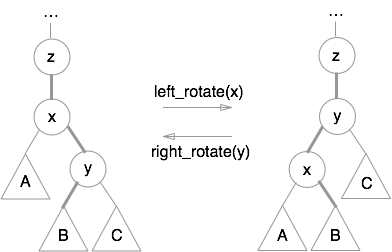
\includegraphics[width=0.42\textwidth]{assets/avl-rotate}
    \end{figure}
  \item Case 1: RR-heavy.
  \item Strategy 1: left rotate the second right-heavy node.
    \begin{figure}[H]
    \centering
    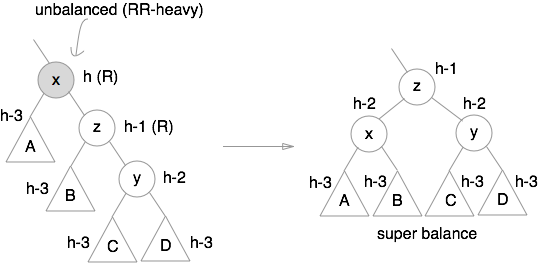
\includegraphics[width=0.48\textwidth]{assets/avl-rr}
    \end{figure}

  \item Case 2: RL-heavy.
  \item Strategy 2: right rotate the left-heavy node and reduce to case 1. Brief: right\_rotate then left\_rotate.
    \begin{figure}[H]
    \centering
    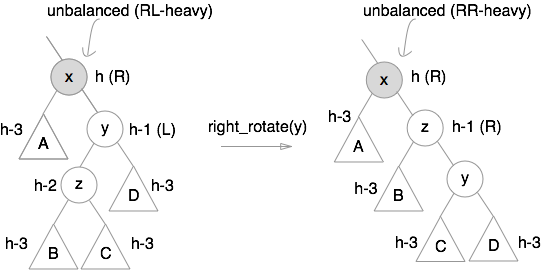
\includegraphics[width=0.48\textwidth]{assets/avl-rl}
    \end{figure}
  
  \item Case 3: LL-heavy.
  \item Strategy 3: right rotate the second left-heavy node.
    \begin{figure}[H]
    \centering
    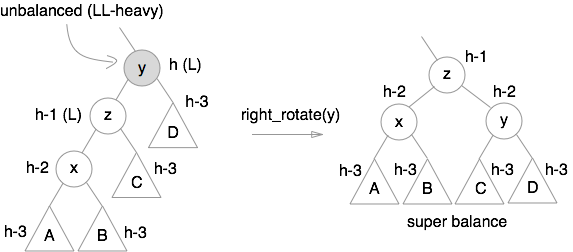
\includegraphics[width=0.48\textwidth]{assets/avl-ll}
    \end{figure}
  
  \item Case 4: LR-heavy.
  \item Strategy 4: left rotate the right-heavy node and reduce to case 3. Brief: left\_rotate then right\_rotate.
    \begin{figure}[H]
    \centering
    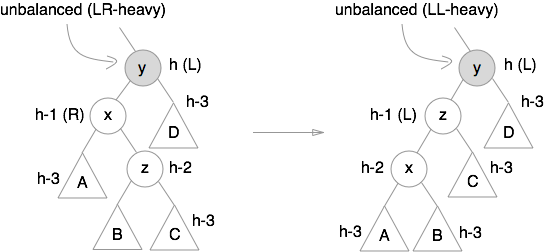
\includegraphics[width=0.48\textwidth]{assets/avl-lr}
    \end{figure}
  \end{itemize}

  \item delete
    \begin{itemize}
    \item Delete as binary search tree.
    \item Unbalance point
      \begin{itemize}
      \item Case 1: the deleted has single left (or nil).
      \item Case 2: the deleted has single right (or nil).
      \item Case 3: the deleted has both children, and the candidate (successor or predecessor depending on the strategy) is not son of it.
      \item Case 4: the deleted has both children, and the candidate is son of it.
      \end{itemize}
      \begin{figure}[H]
      \centering
      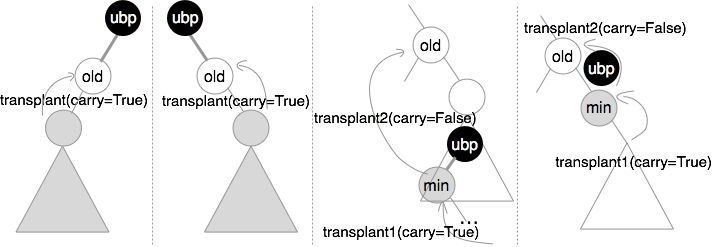
\includegraphics[width=0.48\textwidth]{assets/avl-ubp}
      \end{figure}

    \end{itemize}
\end{itemize}

%%%%

\subsection{Red-black tree}
\begin{itemize}
\item Properties
  \begin{itemize}
  \item All nodes are either red or black.
  \item End nodes are extended with nil leaves.
  \item Root and leaves (nil's) are black.
  \item Red node has black parent.
  \item All simple paths from node $x$ to a leaf have same \# of black nodes.
    \begin{itemize}
      \item black\_height: \# of black's to leaf, excluding start, including leaf.
    \end{itemize}
  \end{itemize}
\item Claim: $h \le 2 \log (n+1)$. Proof:
  \begin{itemize}
  \item Merge red's into black's (2-3-4 tree with height $h'$).
  \item \# leaves = n+1
  \item $2^{h'} \le$ \# leaves $\le 4^{h'}$ 
  \item $h \le 2 h'$
  \end{itemize}
\item insert
  \begin{itemize}
  \item Insert as red node.
  \item Resolve the nodes down to the root.
  \item TODO: cases to switch color or rotate.
  \end{itemize}
\item Versus AVL tree
  \begin{itemize}
  \item More cases to consider.
  \item Asymptotically the same complexity.
  \item Faster insert/delete (fewer rotations).
  \item Slower lookup (greater height).
  \end{itemize}
\end{itemize}

%%%%

\section{Sort}
\begin{itemize}
\item Goal: output $n$ sorted items.
\item Comparison model
  \begin{itemize}
  \item Decision tree: every comparison model can be represented as a decision tree.
  \item \# leaves $\ge$ \# possible outcomes $= n!$
  \item height $\ge \log n! = n \log n - O(n)$ (Sterling).
  \item Lower bound: $\Omega(n \log n)$
  \end{itemize}
\item $O(n \log n)$ sorting
  \begin{itemize}
  \item Quick sort: Pivot. Divide-and-conquer.
  \item Merge sort: Divide-and-conquer.
  \item Heap/BST.
  \end{itemize}
\item Linear-time (integer) sorting
  \begin{itemize}
  \item Counting sort
    \begin{itemize}
    \item L[i]: counter or list of items for integer i.
    \item $O(n+k)$, where $n$ is number of items, $k$ is the largest integer.
    \end{itemize}
  \item Radix sort
    \begin{itemize}
    \item Base $b$ repr: $(\overline{d_{D-1}...d_{1}d_{0}})_b$, where $D=\log_b k$.
    \item Sort each digit by counting sort.
    \item $O((n+b)\log_b k)$
    \item $O(c\,n)$ if $k=n^c$, $b=\Theta(n)$.
    \end{itemize}
  \end{itemize}
\end{itemize}

%%%%%%%%

\section{Order statistics}
\begin{itemize}
\item Find $k$th smallest element.
\item $pivot(p, q, k)$: find $k$th element within $[p, q)$ recursively.
  \begin{itemize}
  \item Worst case: $T(n) = T(n-1) + \Theta(n) = \Theta(n^2)$
  \item Expectation: $E[T(n)] = \Theta(n)$
    \begin{itemize}
    \item $X_i$: indicates if split into $(i, n-i-1)$
    \item $T_i = T(\max \{i, n-i-1\}) + \Theta(n)$
    \item $T(n) = \sum X_i T_i$
    \item $E[T(n)] = \sum_{i=0}^{n-1} T_i / n \le \frac{2}{n} \sum_{i=0}^{\lceil n/2 \rceil} T_i$
    \item $E[T(n)] \le c\,n$ by mathematical induction.
    \end{itemize}
  \end{itemize}
\item Median pivot
  \begin{itemize}
  \item Recursively find median of median.
  \item Choose median of median as pivot.
  \item Partition like above.
  \item $T(n) \le T(\lceil n/5 \rceil) + T(7n/10+6)+O(n)$
  \item $T(n) \le \Theta(n)$ by induction.
  \end{itemize}
  \begin{figure}[H]
  \centering
  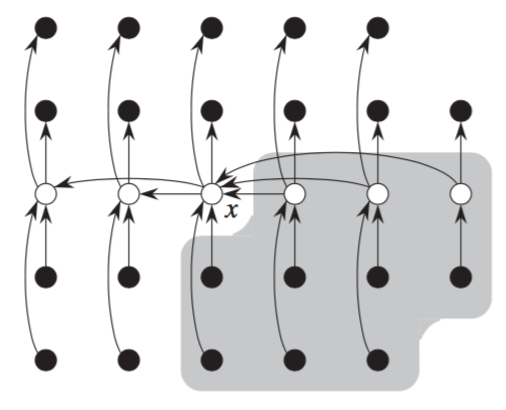
\includegraphics[width=0.28\textwidth]{assets/mpivot}
  \end{figure}
\end{itemize}

%%%%%%%%

\section{Hash}
\begin{itemize}
\item Prehash: map keys to non-negative integers.
\item Hash: map the large key space to smaller space.
\item Chaining: chain up the collided items.
\item Simple uniform hashing
  \begin{itemize}
  \item Assumption: a key is equally likely to be mapped into any slot. The hash value is $r.v.$. This assumption generally does NOT hold true, especially when hash function is determinant.
  \item Load factor $\alpha=n/m$: expected length of chain, where $n$ is \# keys, $m$ is \# slots.
  \item Complexity: $O(1+\alpha)$.
  \end{itemize}
\item Hash functions:
  \begin{itemize}
  \item Mod: $h(k) = k \% m$, where $m$ is prime.
  \item Mul: $h(k) = [(a\cdot k)\,\%\, 2^w]>>(w-r)$, where $w$ is \# bits in $k$ (key), and $r$ is \# bits in $m$ (\# slots).
    \begin{figure}[H]
    \centering
    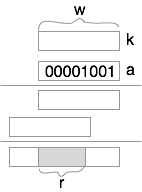
\includegraphics[width=0.18\textwidth]{assets/hash-mul}
    \end{figure}
  \item Universal: $h_{a,b}(k) = [(a\,k+b)\,\%\, p]\,\%\,m$, where $k \in \mathcal{K}$, $p > |\mathcal{K}|$ is picked as prime, and $a,b$ are randomly picked within $\{0,...,p-1\}$.
    \begin{itemize}
    \item ${Pr}\{h_1(k_1)=h_2(k_2)\} = 1/m$, given $k_1, k_2$.
    \end{itemize}
  \end{itemize}
\item Applications
  \begin{itemize}
  \item Dict: random hash + dynamic table
  \item String match: Rabin-Karp
    \begin{itemize}
    \item $h(s) = (\sum ord(s_i) \cdot {base}^i)\,\%\,m$
    \item $h(s_{(i+1):(i+l)}) = \{[h(s_{i:(i+l-1)}) - ord(s_i)] \cdot {base} + ord(s_{i+l})\}\,\%\,m$
    \end{itemize}
  \end{itemize}
\end{itemize}

\subsection{Universal hashing}
\begin{itemize}
\item Adversary model: given hash function is not random, adversary can always find a set of collided keys.
\item Example: $h_{a,b}(k) = [(a\,k+b)\,\%\, p]\,\%\,m$. Each dict is instantiated with different $a$ and $b$.
\item Universal: $|\{h \in \mathcal{H} : h(x) = h(y), x \neq y\}| = |\mathcal{H}|/m$.
  \begin{itemize}
  \item Collision: ${Pr}\{h_1(x)=h_2(y)\} = 1/m$, given $x, y$. 
  \item Theorem: given $x$, $E[\#collisions] < n/m = \alpha$.\\
  Proof: given $h$ is random, denote $r.v.\ C_{x,y} = \mathbb{1}\{h(x)=h(y)\}$, and $C_{x} = \sum_{y \in \mathcal{K}\backslash x} C_{x,y}$, then
    \begin{itemize}
    \item $E[C_{x,y}] = 1/m$
    \item $E[C_x] = \sum_{y \in \mathcal{K} \backslash x} E[C_{x,y}] = \frac{n-1}{m}$
    \end{itemize}
  \end{itemize}
\item Example $h_a(k) = (\sum a_i k_i)\,\%\,m$, where $a=(\overline{a_r..a_1a_0})_m$ and $k = (\overline{k_r..k_1k_0})_m$. Then $|\mathcal{H}| = |\mathcal{K}| = m^{r+1}$.
  \begin{itemize}
  \item Assume $x,y$ differ in $0$th bit, i.e. $x_0 \neq y_0$.
  \item $\sum_{i=0}^r a_i (x_i - y_i) \equiv 0\ (mod\ m)$
  \item $a_0(x_0 - y_0) \equiv -\sum_{i=1}^r a_i (x_i - y_i)\ (mod\ m)$
  \item A theory of Finite (Galois) Field: $\forall z \cancel{\equiv} 0 \in \mathbb{Z}_m, m \in P, then\ \exists z^{-1}, s.t.\ z\,z^{-1} \equiv 1\ (mod\ m)$.
  \item $a_0 \equiv [- \sum_{i=1}^r a_i (x_i - y_i)] (x_0 - y_0)^{-1}\ (mod\ m)$
  \item \# choices to collide at $a_0$: $m^r$ ($a_1..a_r$ are free).
  \end{itemize}
\end{itemize}

%%%%

\subsection{Perfect hashing}
\begin{itemize}
\item Two-level hashing
  \begin{itemize}
  \item Allow $n_i$ collisions in $i$th slot at $1$st level.
  \item Nearly no collision at $2$nd level if \# slots $m_i=n_i^2$.
  \item Worst complexity: $O(1)$.
  \item Theorem: Hash $n$ keys into $m=n^2$ slots using random $h$ in universal hashing would lead to $E[\#collisions] < 1/2$.
    \begin{itemize}
    \item $E[C_{x,y}] = \frac{1}{m} = \frac{1}{n^2}$
    \item $E[C] = \binom{n}{2} \frac{1}{m} = \frac{n-1}{2n} < 1/2$
    \end{itemize}
  \end{itemize}
\end{itemize}

%%%%%%%%

\section{Amortization}
\begin{itemize}
\item Dynamic table
  \begin{itemize}
  \item Grow/shrink the table when necessary.
  \item Load factor $\alpha = n / m$, $n$ is \# items, $m$ is \# slots.
  \item Double the table when $\alpha > \overline{\alpha}$
  \item Shrink the table when $\alpha < \underline{\alpha}$
  \item Aggregate analysis on insertion
    \begin{itemize}
    \item $k$ insertions involve $\log k$ doublings
    \item Doubling cost: $\Theta(2^1+2^2+...+2^{\log k}) = \Theta(k)$
    \item Insertion cost: $\Theta(k)$
    \item Amortized cost: $\frac{1}{k}(\Theta(k)+\Theta(k)) = \Theta(1)$
    \end{itemize}
  \end{itemize}
\item Aggregate method
\item Accounting method
  \begin{itemize}
  \item Charge $i$th op amortized cost $\hat{c}_i$.
  \item Overcharged are stored to bank.
  \item undercharged are taken from bank.
  \item Design charge scheme such that $balance \ge 0$.
  \end{itemize}
\item Potential method
  \begin{itemize}
  \item Design $\Phi_i$ bound with data structure $D_i$.
  \item Requirements: 
    \begin{itemize}
    \item $\Phi_0 = 0$
    \item $\Phi_i \ge 0$, $\forall i$
    \item $\hat{c}_i = c_i + \Phi_i - \Phi_{i-1} \ge 0$
    \end{itemize}
  \item Analyze $\hat{c}_i$ for different cases according to $\Phi_i$.
  \item Any $\Phi_i$ satisfies requirements will do. Better $\Phi_i$ yields tighter upper bound.
  \end{itemize}
\item Example: $\overline{\alpha}=1, \underline{\alpha}=1/4$
  \begin{itemize}
  \item Potential
    \begin{empheq}[left={\Phi_i=\empheqlbrace}]{align*}
      2 n_i - m_i &\quad, \alpha_i \ge 1/2
      \\
      n_i/2 - m_i &\quad, \alpha_i < 1/2
    \end{empheq}
  \end{itemize}
\end{itemize}

%%%%%%%%

\section{Numbers}
\subsection{Catalan numbers}
\begin{itemize}
\item Def
  \begin{itemize}
  \item P: set of balanced parentheses.
  \item $\perp \in P$ ($\perp$ means empty).
  \item If $\alpha, \beta \in P$, then $(\alpha)\beta \in P$.
  \end{itemize}
\item $C_n = |P_n|$ with $n$ pairs of parentheses.
  \begin{itemize}
  \item $C_0 = C_1 = 1$.
  \item $C_{n+1} = \sum_{k=0}^n C_k C_{n-k}$
  \end{itemize}

\end{itemize}

%%%%

\subsection{High precision}
\begin{itemize}
\item Newton's method
  \begin{itemize}
  \item Tangent on $x_i$: $y = f(x_i) + f'(x_i) (x-x_i)$
  \end{itemize}
\item Square root
  \begin{itemize}
  \item $x = \sqrt{a} \Rightarrow
  f(x) = x^2 - a = 0$
  \item $x_{i+1} = x_i - f(x_i)/f'(x_i) = (x_i + a/x_i) / 2$
  \item Quadratic convergence: \# $\checkmark$ digits $\propto$ (\# iters)$^2$
  \end{itemize}
\item Multiplication (Karatsuba)
  \begin{itemize}
  \item $z = x \, y$
  \item $x = x_1\,r^{n/2} + x_0$
  \item $z = z_0 + z_2 + z_1$
    \begin{itemize}
    \item $z_0 = x_0\,y_0$
    \item $z_2 = x_2\,y_2$
    \item $z_1 = (x_0 + x_1) (y_0 + y_1) - z_0 - z_2$
    \end{itemize}
  \item $T(n) = 3 T(n/2) + \Theta(n) = \Theta(n^{\log 3}) \approx \Theta(n^{1.58})$
  \end{itemize}
\item Advanced multiplication
  \begin{itemize}
  \item gmpy2
  \item Schonhage-Strassen: FFT, $\Theta(n\,\lg n\,\lg\lg n)$.
  \item Furer: $\Theta(n\,\log n\,2^{O(\log^* n)})$
  \end{itemize}
\item Division
  \begin{itemize}
  \item $x = R/b \Rightarrow f(x) = 1/x - b/R = 0$
  \item $x_{i+1} = 2 x_i - b x_i^2 / R$
  \item $R = (\overline{r_{d-1}..r_1r_0})_2$, power of 2 is easy to divide.
   \item $T(n) = O(\lg n\, n^{\alpha})$, break down to mul's.
  \end{itemize}
\item When precision digits grow large, complexity of mul, div, sqrt becomes nearly the same as $O(n^{\alpha})$.
\end{itemize}

%%%%%%%%

\section{Graph}
\begin{itemize}
\item Edge
  \begin{itemize}
  \item Tree edge: $old \rightarrow new$
  \item Forward edge: given path $x_0 \rightarrow ... \rightarrow x_n$, any edge not in the path that points to descendant.
  \item Backward edge: ..., to ascendant.
  \item Cross edge: Between subtrees.
  \item Undirected G can have tree edges and back edges.
  \end{itemize}
\item Search
  \begin{itemize}
  \item Breadth first search (BFS)
  \item Depth first search (DFS)
  \end{itemize}
\item Min span tree (DFS/BFS): search and save edges.
\item Cyclic detection (DFS): find back edges.
  \begin{itemize}
  \item Back edge: Edge($v_2 \rightarrow v_1$), $v_1$ is ascendant.
  \item $v_1$ is ascendant of $v_2$ if $(t_1^{in}, t_1^{out}) \supset (t_2^{in}, t_2^{out})$.
  \item Practically we also need to check if $v_1$ and $v_2$ have the same root. It is possible that we first DFS $v_1$, and then $v_2$.
  \end{itemize}
\item Topological sort (DFS):
  \begin{itemize}
  \item Append the out nodes.
  \item Reverse the order.
  \end{itemize}
\item Dependency management (DFS):
  \begin{itemize}
  \item Reverse edges and run topological sort.
  \end{itemize}
\end{itemize}

%%%%

\subsection{Dijkstra}
\begin{itemize}
\item Single source shortest path
\item Do NOT allow negative weights
\item Outputs
  \begin{itemize}
  \item $d[v]$: shortest distance from source to $v$.
  \item $p[v]$: parent of $v$ in the shortest path.
  \end{itemize}
\item Dynamic programming
  \begin{itemize}
  \item $S$ is safe set, within which have been reached by shortest path from source.
  \item $R$ is the remaining set.
  \end{itemize}
\item Optimize
  \begin{itemize}
  \item Maintain $d$ as priority queue, so that each time \textit{EXTRACT-MIN} only takes $O(\log|V|)$
  \item Total complexity: $O(|E|+|V|\log|V|)$
  \end{itemize}
\item Single source single destination
  \begin{itemize}
  \item $S_f$ forward safe set.
  \item $S_b$ backward safe set.
  \item Stop when two sets intersect.
  \end{itemize}
\end{itemize}

%%%%

\subsection{Bellman-Ford}
\begin{itemize}
\item Single source shortest path that allows negative weights.
\item Mark $d[v]=-\text{inf}$ to indicate negative cycle.
\item Algorithm
  \begin{itemize}
  \item Relax ALL edges for $|V|-1$ passes.
  \item Relax one more time to check negative cycle.
  \end{itemize}
\item Complexity $O(|V||E|)$.
\end{itemize}

%%%%%%%%

\section{Misc}


%%%%%%%%

\end{document}